\section{Les stratégies d'échanges impliquant des options}

Les options peuvent être combinées entre elles ou avec l'actif sous-jacent pour créer des stratégies d'investissement adaptées à différents scénarios de marché (hausse, baisse, stabilité ou volatilité).

\subsection{Stratégies impliquant une option et un actif sous-jacent}

La stratégie la plus emblématique de cette catégorie est la \textbf{vente de call couvert} (ou \textit{covered call}).

\begin{definitionbox}[Covered Call]
Cette stratégie consiste à détenir une position longue sur l'action (achat du sous-jacent) tout en prenant simultanément une position courte sur un call (vente d'une option d'achat) sur ce même actif.
\end{definitionbox}

\begin{intuitionbox}[Mécanisme du Covered Call]
Le terme "couvert" vient du fait que l'investisseur possède déjà l'action qu'il pourrait être obligé de livrer si l'option est exercée par l'acheteur.
\begin{itemize}
    \item \textbf{Avantage :} L'investisseur encaisse la prime de l'option, ce qui améliore son rendement si l'action stagne ou monte modérément. Cette prime offre également une légère protection (un "coussin") en cas de baisse du cours de l'action.
    \item \textbf{Inconvénient :} En échange de la prime reçue, l'investisseur renonce à tout profit potentiel lié à une hausse du cours de l'action au-delà du prix d'exercice ($K$). Son gain est plafonné.
\end{itemize}
\end{intuitionbox}

\begin{center}
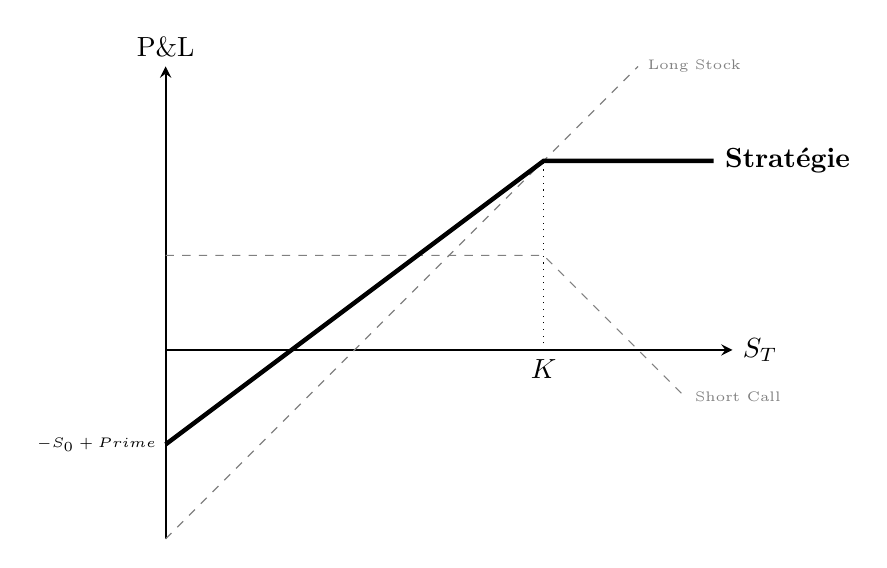
\begin{tikzpicture}[scale=1.2]
    % Axes
    \draw[->, >=stealth, thick] (0,-2) -- (0,3) node[above] {P\&L};
    \draw[->, >=stealth, thick] (0,0) -- (6,0) node[right] {$S_T$};
    
    % Composantes (Lignes pointillées)
    \draw[dashed, gray] (0,-2) -- (5,3) node[right] {\tiny Long Stock};
    \draw[dashed, gray] (0,1) -- (4,1) -- (5.5,-0.5) node[right] {\tiny Short Call};
    
    % Courbe de la stratégie (Trait noir épais)
    \draw[ultra thick, black] (0,-1) -- (4,2) -- (5.8,2) node[right] {\bfseries Stratégie};
    
    % Annotations
    \draw[dotted] (4,0) node[below] {$K$} -- (4,2);
    \node[left, font=\tiny] at (0,-1) {$-S_0 + Prime$};
\end{tikzpicture}
\end{center}

\subsection{Les Spreads}

Un spread est une stratégie combinant l'achat et la vente d'options de même type (deux calls ou deux puts) sur le même sous-jacent.

\subsubsection{Le Bull Spread (Spread Haussier)}

Comme son nom l'indique, cette stratégie est utilisée lorsque l'investisseur anticipe une hausse du marché.

\textbf{Construction avec des Calls :}
Un bull spread standard est créé en achetant un call à un prix d'exercice bas ($K_1$) et en vendant un call à un prix d'exercice plus élevé ($K_2$).
Puisque le call $K_1$ (plus proche du cours ou dans la monnaie) est plus cher que le call $K_2$ (hors de la monnaie), cette stratégie nécessite un \textbf{investissement initial} (débit).

\textbf{Profil de gain :}
\begin{itemize}
    \item Si le cours finit sous $K_1$ : Les deux options expirent sans valeur. La perte est limitée à l'investissement initial.
    \item Si le cours finit au-dessus de $K_2$ : Le gain sur le call acheté est plafonné par la perte sur le call vendu. Le profit est maximal et constant.
\end{itemize}

% --- GRAPHIQUE BULL SPREAD (Nettoyé + Composants ajoutés) ---
\begin{center}
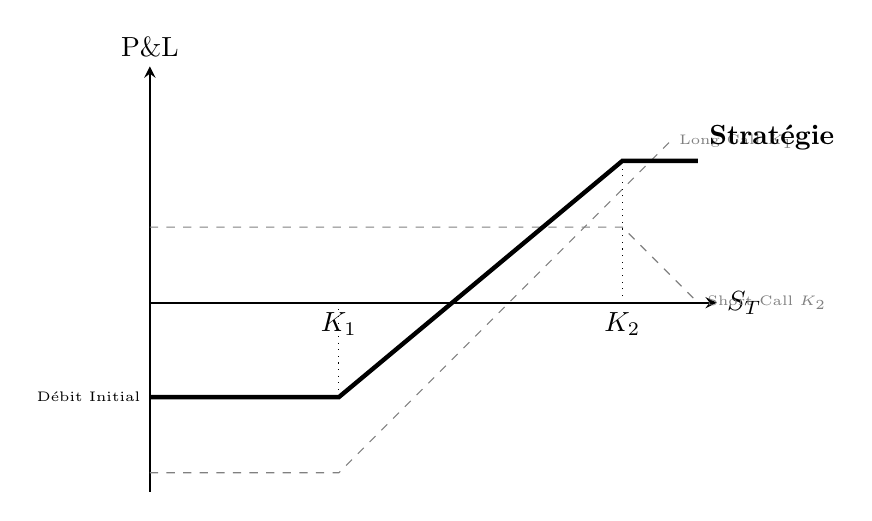
\begin{tikzpicture}[scale=1.2]
    % Axes
    \draw[->, >=stealth, thick] (0,-2) -- (0,2.5) node[above] {P\&L};
    \draw[->, >=stealth, thick] (0,0) -- (6,0) node[right] {$S_T$};
    
    % Composantes ajoutées (Visuelles/Illustratives)
    % Long Call K1 (Coût plus élevé, donc départ plus bas)
    \draw[dashed, gray] (0,-1.8) -- (2,-1.8) -- (5.5,1.7) node[right, font=\tiny] {Long Call $K_1$};
    % Short Call K2 (Crédit reçu, donc départ positif)
    \draw[dashed, gray] (0,0.8) -- (5,0.8) -- (5.8,0) node[right, font=\tiny] {Short Call $K_2$};

    % Stratégie
    \draw[ultra thick, black] (0,-1) -- (2,-1) -- (5,1.5) -- (5.8,1.5) node[above right] {\bfseries Stratégie};
    
    % Annotations
    \draw[dotted] (2,0) node[below] {$K_1$} -- (2,-1);
    \draw[dotted] (5,0) node[below] {$K_2$} -- (5,1.5);
    \node[left, font=\tiny] at (0,-1) {Débit Initial};
\end{tikzpicture}
\end{center}

\begin{remarquebox}[Bull Spread avec Puts]
Un bull spread peut également être construit en achetant un put avec un prix d'exercice bas ($K_1$) et en vendant un put avec un prix d'exercice plus élevé ($K_2$). Contrairement à la version avec calls, cette combinaison génère un \textbf{flux initial positif} (crédit), car le put vendu ($K_2$) vaut plus cher que le put acheté ($K_1$). Le profil de risque à l'échéance reste similaire (profit si le marché monte).
\end{remarquebox}

\subsubsection{Le Bear Spread (Spread Baissier)}

Le bear spread est la stratégie miroir, utilisée lorsque l'on anticipe une baisse du cours de l'action.

\textbf{Construction avec des Puts :}
On achète un put à un prix d'exercice élevé ($K_2$) et on vend un put à un prix d'exercice plus bas ($K_1$).
Cette stratégie a un coût initial, mais permet de profiter de la baisse jusqu'au niveau $K_1$.

\textbf{Construction avec des Calls :}
On vend un call à un prix d'exercice bas ($K_1$) et on achète un call à un prix d'exercice élevé ($K_2$).
L'investisseur reçoit une prime nette au départ (crédit). Si le marché baisse, il conserve cette prime comme profit maximal. Si le marché monte, ses pertes sont limitées par le call acheté qui agit comme une assurance.

\subsection{Les Butterfly Spreads}

Le butterfly spread est une stratégie de volatilité neutre. Elle implique des positions sur trois prix d'exercice différents, généralement espacés de manière symétrique : $K_1 < K_2 < K_3$.

\begin{definitionbox}[Construction du Butterfly]
Pour créer un butterfly spread en utilisant des calls :
\begin{itemize}
    \item Achat d'un call au prix d'exercice bas $K_1$.
    \item Achat d'un call au prix d'exercice élevé $K_3$.
    \item Vente de \textbf{deux} calls au prix d'exercice intermédiaire $K_2$ (généralement proche du cours actuel $S_0$).
\end{itemize}
\end{definitionbox}

\begin{intuitionbox}[Profil de gain]
Cette stratégie produit un bénéfice maximal si le cours de l'action à l'échéance reste proche de $K_2$. C'est une stratégie de "stabilité".
\begin{itemize}
    \item Si l'action varie significativement (très bas en dessous de $K_1$ ou très haut au-dessus de $K_3$), la stratégie conduit à une perte faible et limitée (égale au coût de mise en place de la stratégie).
    \item Le graphique de gain ressemble à un triangle (ou aux ailes d'un papillon) avec un pic en $K_2$.
\end{itemize}
\end{intuitionbox}

\begin{center}
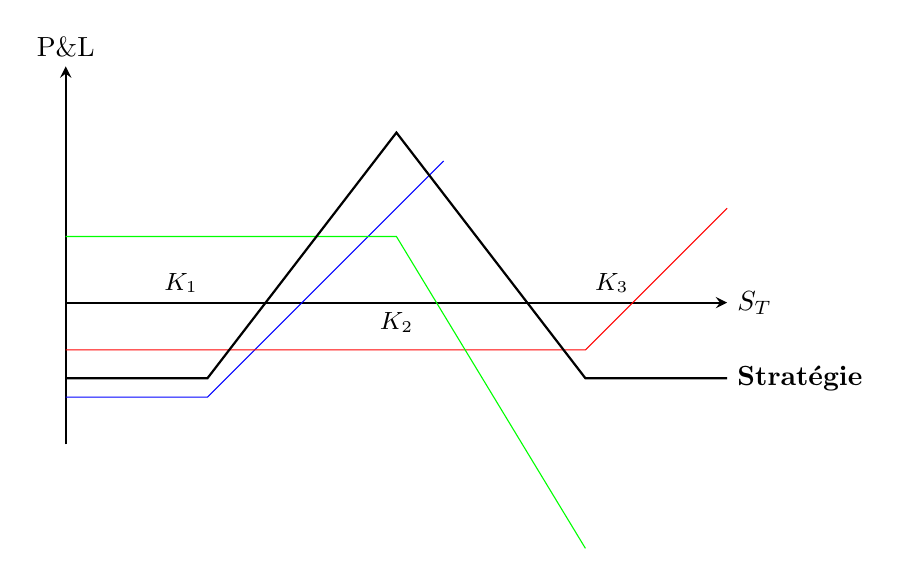
\begin{tikzpicture}[scale=1.2]
    \draw[->, >=stealth, thick] (0,-1.5) -- (0,2.5) node[above] {P\&L};
    \draw[->, >=stealth, thick] (0,0) -- (7,0) node[right] {$S_T$};
    
    \draw[blue] (0,-1) -- (1.5,-1) -- (4,1.5); 
    \draw[red] (0,-0.5) -- (5.5,-0.5) -- (7,1); 
    \draw[green] (0,0.7) -- (3.5,0.7) -- (5.5,-2.6);
    
    \draw[thick, black] (0,-0.8) -- (1.5,-0.8) -- (3.5,1.8) -- (5.5,-0.8) -- (7,-0.8) node[right] {\bfseries Stratégie};
    
    \node[above left, font=\small] at (1.5,0) {$K_1$};
    \node[below, font=\small] at (3.5,0) {$K_2$};
    \node[above right, font=\small] at (5.5,0) {$K_3$};

\end{tikzpicture}
\end{center}

\subsection{Le Straddle (Stellage)}

Le Straddle est une stratégie purement orientée vers la volatilité. Elle est utilisée lorsqu'un investisseur s'attend à un mouvement violent du cours de l'action, mais ignore dans quelle direction ce mouvement se produira (par exemple, avant l'annonce de résultats d'entreprise incertains).

\begin{definitionbox}[Construction du Straddle]
Un \textbf{Long Straddle} consiste à acheter simultanément :
\begin{itemize}
    \item Un Call au prix d'exercice $K$.
    \item Un Put au même prix d'exercice $K$.
\end{itemize}
Les deux options doivent avoir la même date d'échéance.
\end{definitionbox}

\begin{intuitionbox}[Profil de Risque/Rendement]
Cette stratégie nécessite un investissement initial important (somme des primes du Call et du Put).
\begin{itemize}
    \item \textbf{Perte maximale :} Limitée au coût des primes. Elle survient si le cours de l'action finit exactement à $K$ (les deux options expirent sans valeur).
    \item \textbf{Gain :} Il est potentiellement illimité. Pour être rentable, l'action doit s'éloigner suffisamment de $K$ (à la hausse ou à la baisse) pour couvrir le coût des deux primes. Le profil de gain forme un "V".
\end{itemize}
\end{intuitionbox}

\begin{center}
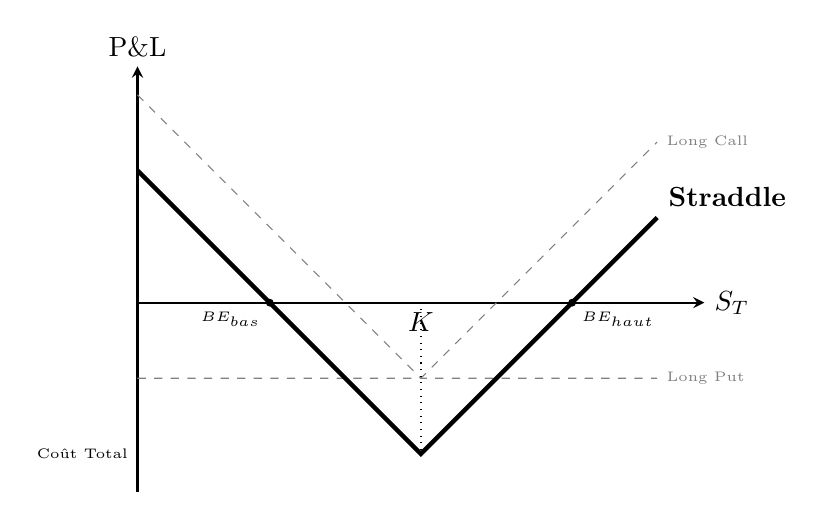
\begin{tikzpicture}[scale=1.2]
    % Axes
    \draw[->, >=stealth, thick] (0,-2) -- (0,2.5) node[above] {P\&L};
    \draw[->, >=stealth, thick] (0,0) -- (6,0) node[right] {$S_T$};
    
    % Composantes (Lignes pointillées grises)
    % Call
    \draw[dashed, gray] (0,-0.8) -- (3,-0.8) -- (5.5,1.7) node[right, font=\tiny] {Long Call};
    % Put
    \draw[dashed, gray] (0,2.2) -- (3,-0.8) -- (5.5,-0.8) node[right, font=\tiny] {Long Put};
    
    % Stratégie (Trait noir épais)
    % Somme des deux primes = -1.6 (arbitraire pour le dessin)
    \draw[ultra thick, black] (0,1.4) -- (3,-1.6) -- (5.5,0.9) node[above right] {\bfseries Straddle};
    
    % Annotations
    \draw[dotted] (3,0) node[below] {$K$} -- (3,-1.6);
    \node[left, font=\tiny] at (0,-1.6) {Coût Total};
    
    % Break-even points (approximatifs visuellement)
    \draw[fill=black] (1.4,0) circle (1pt) node[below left, font=\tiny] {$BE_{bas}$};
    \draw[fill=black] (4.6,0) circle (1pt) node[below right, font=\tiny] {$BE_{haut}$};
\end{tikzpicture}
\end{center}

\subsection{Le Strangle}

Le Strangle est une variante du Straddle, également utilisée pour parier sur la volatilité, mais avec un coût d'entrée plus faible.

\begin{definitionbox}[Construction du Strangle]
Un \textbf{Long Strangle} consiste à acheter deux options \textit{hors de la monnaie} (Out-of-the-Money) :
\begin{itemize}
    \item Un Put avec un prix d'exercice bas $K_1$.
    \item Un Call avec un prix d'exercice plus élevé $K_2$ (avec $K_1 < K_2$).
\end{itemize}
\end{definitionbox}

\begin{intuitionbox}[Différence avec le Straddle]
Comme les deux options sont achetées "hors de la monnaie", leurs primes sont moins chères que celles d'un Straddle (qui utilise des options "à la monnaie").
\begin{itemize}
    \item \textbf{Avantage :} Le coût initial est plus faible, donc la perte maximale est réduite.
    \item \textbf{Inconvénient :} Pour être rentable, l'action doit faire un mouvement \textbf{encore plus important} que pour un Straddle. Le cours doit dépasser $K_2$ ou passer sous $K_1$ de manière significative.
\end{itemize}
\end{intuitionbox}

\begin{center}
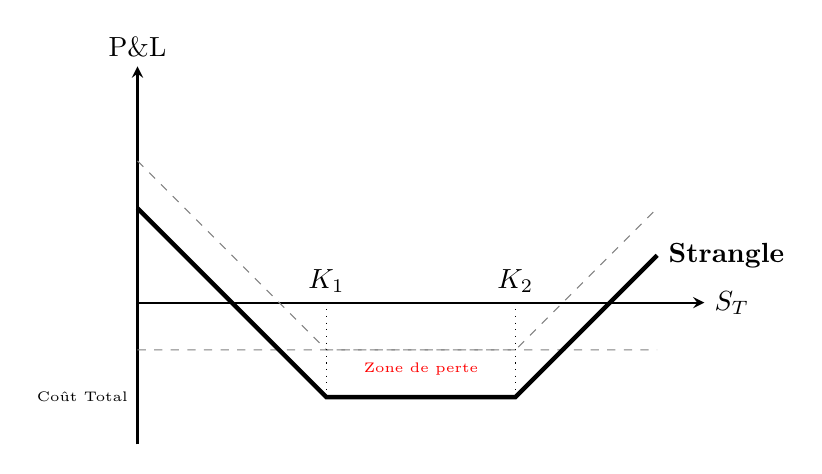
\begin{tikzpicture}[scale=1.2]
    % Axes
    \draw[->, >=stealth, thick] (0,-1.5) -- (0,2.5) node[above] {P\&L};
    \draw[->, >=stealth, thick] (0,0) -- (6,0) node[right] {$S_T$};
    
    % Composantes (Lignes pointillées grises)
    % Long Put K1
    \draw[dashed, gray] (0,1.5) -- (2,-0.5) -- (5.5,-0.5);
    % Long Call K2
    \draw[dashed, gray] (0,-0.5) -- (4,-0.5) -- (5.5,1);
    
    % Stratégie (Trait noir épais)
    % Coût total = -1.0 (somme des deux primes plus faibles)
    \draw[ultra thick, black] (0,1) -- (2,-1) -- (4,-1) -- (5.5,0.5) node[right] {\bfseries Strangle};
    
    % Annotations
    \draw[dotted] (2,0) node[above] {$K_1$} -- (2,-1);
    \draw[dotted] (4,0) node[above] {$K_2$} -- (4,-1);
    \node[left, font=\tiny] at (0,-1) {Coût Total};
    
    % Zone de perte
    \node[font=\tiny, text=red] at (3,-0.7) {Zone de perte};

\end{tikzpicture}
\end{center}